\documentclass[a4paper,14pt]{article}
\usepackage[utf8]{inputenc}
\usepackage[russian]{babel} 
\usepackage{graphicx} 
\usepackage{amsmath}
\usepackage{amssymb}
\usepackage{float}
\usepackage[colorlinks=true, linkcolor=blue]{hyperref}
\usepackage{enumitem}

\renewcommand{\floatpagefraction}{0.99}
\renewcommand{\topfraction}{0.99}      



\title{ ЛАБОРАТОРНАЯ РАБОТА №2.1.
Электроизмерительные приборы и источники питания постоянного тока}


\author{Батанин Артём Александрович}
\date{\today}


\begin{document}

\maketitle

\newpage
\tableofcontents    
\newpage            



\section{Цель работы}
Цель работы – познакомиться с устройством, принципом действия электромеханических и цифровых измерительных приборов; 
научиться проводить измерения тока и напряжения в цепях постоянного тока, а также с режимами работы источников питания постоянного тока.


\section{Задание 1. Изучение влияния вольтметра на режим
работы электрической цепи постоянного тока}

Оборудование: вольтметр магнитоэлектрической системы
М2044 (или аналогичный); цифровой мультиметр серии GDM-8145;
источник питания постоянного тока Б5-47; панель с делителем на-
пряжения.

\begin{figure}[h!]
\centering
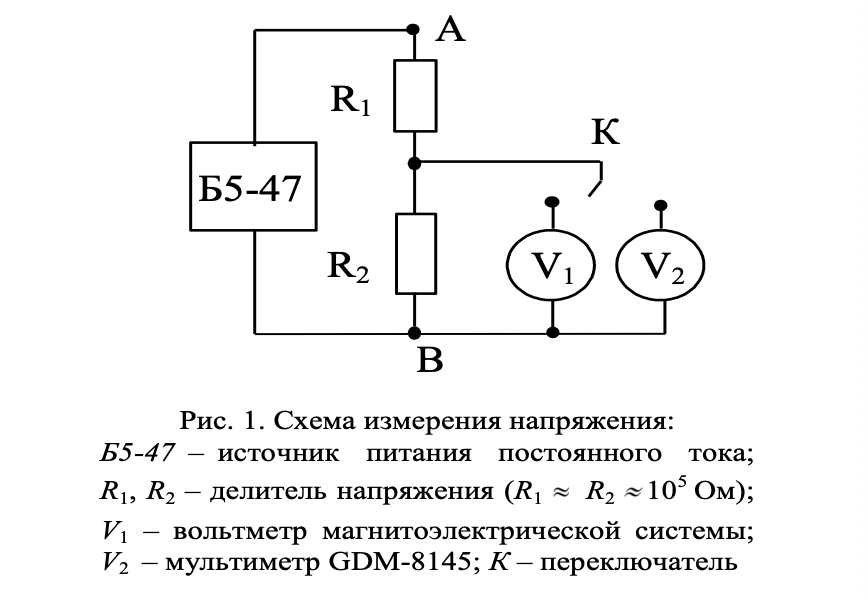
\includegraphics[width=1\linewidth]{schema1.png}
\label{fig:schema1}
\
\end{figure}


\begin{table}[htbp]
  \centering
  \caption{Пример простой таблицы}
  \label{tab:my_label}
  \begin{tabular}{|c|c|c|c|c|c|c|c|}
    \hline
    Вольтметр & Шкала, В & U, В & dU, В & $U_{0}, B$  & $R_v$, Ом & \multicolumn{2}{|c|}{U, В при параллельном соединении}    \\ \hline
    GDM & 20 & 0 & 0 & 0 & 0 & M2044 & GDM \\ \hline
    M2044 & 75 & 0 & 0 & 0 & 0 & 0 & 0 \\ \hline
    M2044 & 30 & 0 & 0 & 0 & 0 & 0 & 0 \\ \hline
    M2044 & 15 & 0 & 0 & 0 & 0 & 0 & 0 \\ \hline

  \end{tabular}
\end{table}






\newpage 

\section{Графики и результаты}





\end{document}